The last prototype developed in TRITIUM experiment and the second thought to be the final versión of the TRITIUM detector module was TRITIUM-IFIC 2, which is shown in Figure \ref{fig:TritiumIFIC2}, A.

\begin{figure}[h]
\centering
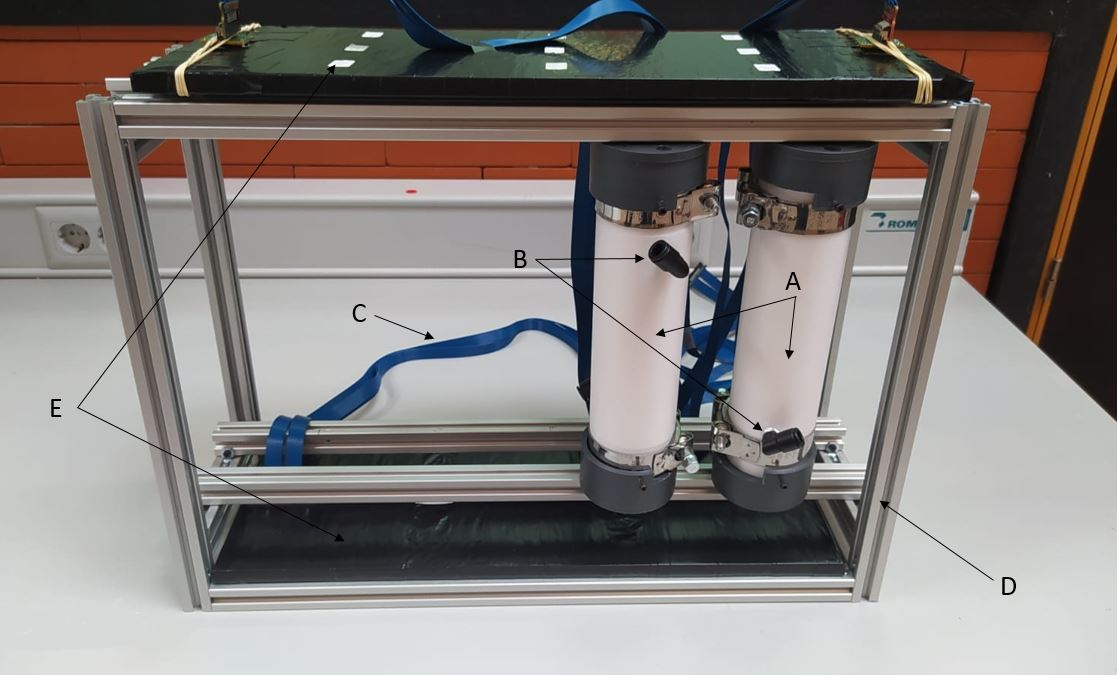
\includegraphics[scale=0.4]{5Prototypes/53FinalPrototypes/532TritiumIFIC2/Tritium_IFIC_2_full_module.jpg}
\caption{TRITIUM-IFIC 2 prototype.\label{fig:TritiumIFIC2}}
\end{figure}

This prototype was designed and built in the IFIC workshop and it consists of a cylindrical teflon vessel, shown in Figure \ref{fig:Tritium-IFIC2_vessels}, the shape of which is similar to the one used in TRITIUM-Aveiro 0 prototype The internal length and diameter of the teflon vessel are $200~\mm$ and $36~\mm$ respectively.

\begin{figure}
\centering
    \begin{subfigure}[b]{0.35\textwidth}
    \centering
    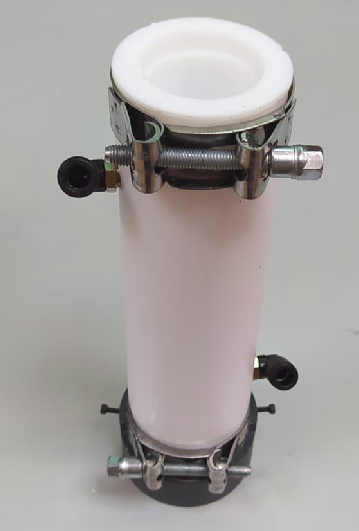
\includegraphics[width=\textwidth]{5Prototypes/53FinalPrototypes/532TritiumIFIC2/Tritium_IFIC_2_vessel1.png}  
    \caption{TRITIUM-IFIC 2 vessel.\label{subfig:Tritium_IFIC_2_vessel}}
    \end{subfigure}
    \hfill
    \begin{subfigure}[b]{0.3\textwidth}
    \centering
    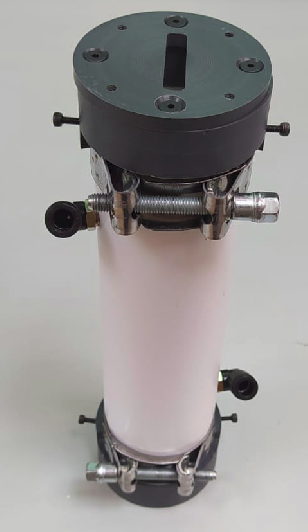
\includegraphics[width=\textwidth]{5Prototypes/53FinalPrototypes/532TritiumIFIC2/Tritium_IFIC_2_vessel2.png}  
    \caption{TRITIUM-IFIC 2 vessel with PVC caps.\label{subfig:TritiumIFIC2_vessel_with_PVC_caps}}
    \end{subfigure}
 \caption{TRITIUM-IFIC 2 teflon vessel.}
 \label{fig:Tritium-IFIC2_vessels}
\end{figure}

This prototype contains $800$ no-clad scintillating fibers, model BCF-12, with a length of $200~\mm$, a larger number of fibers than the TRITIUM-Aveiro 0 prototype which are arranged in less volume.

The fibers used are cut, polished and cleaned with the conditioning processes previously shown in section \ref{sec:CharacterizationScintillatingFibers} since, during the construction of the prototype, the development of the automatic polishing machine was completed.

These fibers are freely arranged, with a density that allows water to flow through the fibers and two PMMA windows located at the ends of the fiber bundle were used to read this system, similar to the TRITIUM-Aveiro 0 prototype. 

The width of the PMMA optical windows used is $5~\mm$, which is sufficient to guarantee radiosecurity since the detector works at very low water pressure and two clamps are used to ensure the watertightness of the prototype, similar to the TRITIUM-Aveiro 0 prototype. The transmission coefficient, shown in Figure \ref{fig:PMMATransmissionSpectrum}, is practically unaffected by the little difference of the PMMA width used in both prototypes.

As can be seen in Figure \ref{fig:TritiumIFIC2}, B, and Figure \ref{fig:Tritium-IFIC2_vessels}, a water inlet/outlet was installed in the teflon vessel to allow a constant water flux through it, similar to the TRITIUM-Aveiro 0 prototype.

For the first laboratory measurements, two PMTs were used, model R8520-460 from the Hamamatsu Photonics company \cite{DataSheetPMTs}, which is useful to understand the results and compare them with the results obtained with the previous prototypes. However, measurements with SiPM arrays have already started the output signal of which is connected to PETSYS system through flat wires as can be seen in Figure \ref{fig:TritiumIFIC2}, C.

As SiPM arrays readout by the PETSYS system will be employed in the TRITIUM-IFIC 2 prototype that will be installed in Arrocampo dam, it is not necessary to develop a electronics chain to process and analyze the PMT signals of this prototype.

Like the TRITIUM-Aveiro 0 prototype, although PETSYS has a graphical user interface, shown in Figure \ref{fig:GUI_PETSYS}, which allows controlling all the different options such as the voltage with which the SiPM arrays is fed, the thresholds used, etc., normally it will be controlled remotely via computer terminal. 

\begin{figure}[h]
\centering
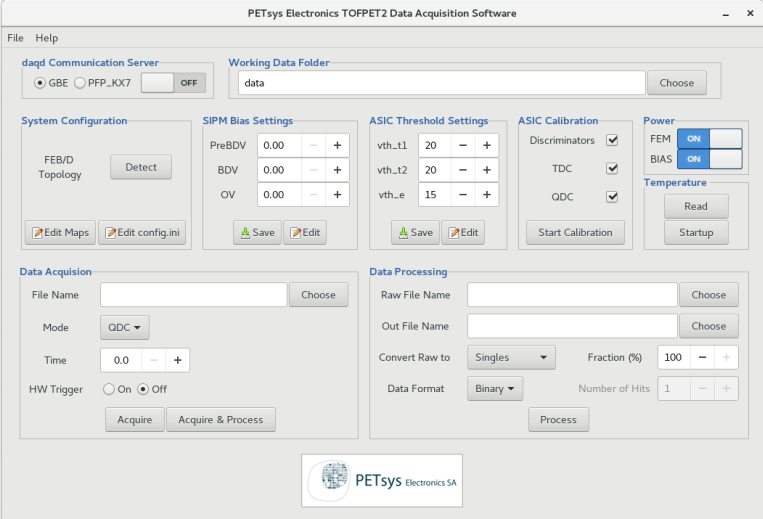
\includegraphics[scale=0.4]{5Prototypes/53FinalPrototypes/532TritiumIFIC2/GUI_PETSYS.png}
\caption{Graphical User Interface (GUI) of PETSYS.\label{fig:GUI_PETSYS}}
\end{figure}

Two PVC caps, located at both ends of the prototype, Figure \ref{subfig:TritiumIFIC2_vessel_with_PVC_caps}, were used to work with the SiPMs in a light-tight environment and an aluminum structure, shown in Figure \ref{fig:TritiumIFIC2}, was designed and built to house up to 10 TRITIUM-IFIC 2 modules and two cosmic vetos, shown in Figure \ref{fig:TritiumIFIC2}, E.

The available space of the lead shielding, explained in section \ref{subsec:SetUpPassiveShield} is enough to accommodate up to 5 structures like the one shown in Figure \ref{fig:TritiumIFIC2}. It means that the final TRITIUM module has the capacity to contains 50 TRITIUM-IFIC 2 modules and 10 different cosmic vetos. As the sensibility of the TRITIUM monitor scales with the number of TRITIUM modules used, the results obtained with the TRITIUM monitor can improve the results obtained with the TRITIUM-IFIC 2 prototype by a factor of N, where N is the number of cells used.

Two identical TRITIUM-IFIC 2 prototypes were built, similar to the TRITIUM-IFIC 0 prototype, one of them was filled with ultrapure water and used to measure the background and the other was filled with a radioactive liquid source of tritium and used to measure the signal. The volume used in both cases was $82~\milli\liter$ (uncertainty of $0.05\%$).

The activity of the tritium source used for this prototype is $10~\kilo\becquerel/\liter$ (uncertainty of $2.24\%$), which was prepared by diluting a sample of tritiated water explained in appendix \ref{App:TritiumSourcePreparation} with ultrapure water until the desired activity was achieved.

The results of this prototype is shown in section \ref{subsec:ResultsTritiumIFIC2}, where they are compared with the results of the previous prototypes and, specially, with TRITIUM-Aveiro 0 prototype.